\chapter{Linear Models}

We now move over to discuss another simple model in Machine Learning, the class of \textbf{Linear Models}. Linear Models leads us to the introduction of \textbf{perceptrons}.

Some machine learning approaches make strong assumptions about the data: if the assumptions are true it can often lead to better performance, but if the assumptions are false the approach can fail miserably.
Other approaches don't make many assumptions about the data, this can allow us to learn from more varied data, but they are more prone to overfitting and generaly require more training data.

Linear models generate a formula to create a best-fit line to predict unknown values. Linear Models are considered not as predictive as newer algorithm classes, but they can be trained relatively quicky and are generally more straightforward to interpret, which can be a big plus.

\section{Bias}
The \textbf{bias} of a model is how strong the model assumptions are. Low-bias classifiers make minimal assumptions about the data (kNN and decision trees are generally considered low bias), high-bias classifiers make strong assumptions about the data.

A strong high-bias assumption is \textbf{linear separability}: in two dimenstions, can separate classes by a line, in higher dimensions, need hyperplanes.

A linear model is a model that assumes the data is linearly separable.

\subsection{Define a line}
Any pair of values \((w_1,w_2)\) defines a line through the origin: \(w_1f_1 + w_2f_2 = 0\).

\begin{example}
\begin{wrapfigure}{l}{0.25\textwidth}
\begin{center}
    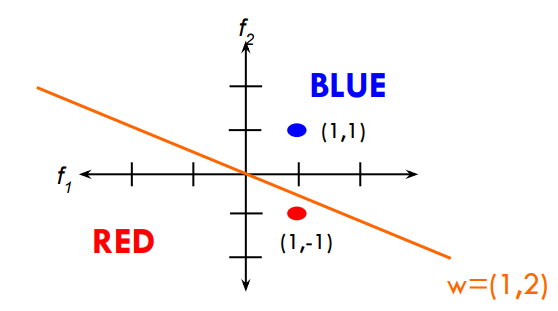
\includegraphics[width=0.25\textwidth]{031}
    \label{fig:031}
\end{center}
\caption{}
\end{wrapfigure}
For example, in Figure~\ref{fig:031} we have the line \(1f_1+2_2 = 0\). This equation means that we have our training data in a two-dimensional space, we have only two features (\(f_1\) and \(f_2\)), and the line that separate our training points is the orange line.

We can see the parameters \((w_1=1,w_2=2)\) as the vector perpendicular to the orange line. In fact, the orange line is perpendicular to the vector that starts from the origin \(O(0,0)\), and goes to the point \(w(1,2)\).

How can we classify mathematically the points based on a line? If we got two example data \(B(1,1)\) and \(R(1,-1)\), we have the following results:
\begin{align*}
(1,1) &: 1*1+2*1=3\\
(1,-1) &: 1*1+2*(-1)=-1
\end{align*}
The sign of the result indicates which side of the line is occupied by the example in the space.

\end{example}

We can move our line from the origin, if we use the following equation, that uses a parameter \(a\) in order to represent any line in a two dimensional space:
\[w_1f_1+w_2f_2=a\]
In this case we have a line intersects at \(a\) in the horizontal axis.

A linear model in \(n\)-dimensional space (i.e. \(n\) features) is defined by \(n+1\) weights. In two dimesions, we have a line 
\begin{equation}
    w_1f_1+w_2f_2+b=0 \qquad \text{where } b=-a
\end{equation}
In three dimensions, we have a plane
\[w_1f_1+w_2f_2+w_3f_3+b=0\]
In \(n\) dimensions, we have a \textbf{hyperplane}
\begin{equation}
    b+\sum_{i=1}^nw_if_i=0
\end{equation}

\subsection{Classifying with linear models}
Havin define the notion of line and the notion of hyperplane, we can show that a linear model, and in particular an hyperplane, can be used for classification by simply looking at the sign of the following equation:
\begin{equation}
\label{eqn:001}
b+\sum_{i=1}^nw_if_i
\end{equation}
if the result of equation \ref{eqn:001} is greater than \(0\), we have a positive example that belongs to the positive class; otherwise, if the result is lower than \(0\), we have a negative example that belongs to the negative class.

\section{Online learning}
\textbf{Online learning} is a method of machine learning in which data becomes available in a sequential order ad is used to update the best predictor for future data at each step, as opposed to batch learning techniques which generate the best predictor by learning on the etire training data set at once.

Online learning is able to overcome the drawbacks of batch learning in that the predictive model can be updated intantly for any new data instances. Thus, online learning algorithms are far more efficient and scalable for large-scale machine learning tasks in real-world data analytics applications where data are not only large in size, but also arriving at a high velocity.

\subsection{Tasks and applications}

Online learning algorithms can be derived for supervised learning tasks. One of the most common tasks is classification, aiming to predict the categories for a new data instance belongs to, on the basis of observing past training data instances whose category labels are given. For example, a commonly studied task in online learning is \textbf{online binary classification} (e.g., spam email filtering) which only involves two categories (“spam” vs “benign” emails); other types of supervised classification tasks include multi-class classification, multi-label classification, and multiple-instance classification, etc.

In addition to classification tasks, another common supervised learning task is \textbf{regression analysis}, which refers to the learning process for estimating the relationships among variables (typically between a dependent variable and one or more independent variables). Online learning techniques are naturally applied for regression analysis tasks, e.g., time series analysis in financial markets where data instances naturally arrive in a sequential way. Besides, another application for online learning with financial time series data is \textbf{online portfolio section} where an online learner aims to find a good (e.g., profitable and low-risk) strategy for making a sequence of decisions for portfolio selection.

\section{Perceptron}

The \textbf{perceptron} is an algorithm for supervised learning of binary classifiers. A binary classifier is a function which can decide wheter or not an input, represented by a vectior of numbers, belongs to some specific class. 

In the modern sense, the perceptron is an algorithm for learning a binary classifier called a \text{threshold function}: a function that maps its input \(x\) to an output value \(f(x)\):
\begin{equation}
    f(x) = \begin{cases}
        1               &\text{if \(w \cdot x + b > 0\), } \\
        0               &\text{otherwise}\\
    \end{cases}
\end{equation}
where \(w\) is a vector of real-valued weights, \(w \cdot x\) is the dot product \(\sum_{i=1}^mw_ix_i\), where \(m\) is the number of inputs to the perceptron, and \(b\) is the bias.

The value of \(f(x)\) is used to classify \(x\) as either a positive or a negative instance, in the case of a binary classification problem. If \(b\) is negative, then the weighted combination of inputs must produce a positive value greater thant \(|b|\) in order to push the classifier neuron over the 0 threshold.

Spatially, the bias alters the position of the decision boundary. The perceptron learning algorithm does not terminate if the learning set is not linearly separable. If the vectors are not linearly separable learning will never reach a point where all vectors are classified properly. 

\subsection{Convergence and number of iterations}
We will have convergence when the data are linearly separable, but when data is not linearly separable, we have to set up a number of iterations, otherwise the algorithm will fall in an infinite loop.

The training instances are linearly separable if, given two classes of examples, there exists a hyperplane that will separate the two classes.

The number of iterations can be used to prevent the overfitting of the perceptron algorithm.

\subsection{Algorithm}

\begin{algorithm}
\caption{Perceptron learning}
\label{alg:perceptron}
\While{convergence not reached}{
    \ForEach{training example $f_i$, $label$}{
        $prediction \gets b + \sum_{i=1}^nw_if_i$
        \Comment*[r]{check if it is correct}
        \If{not correct}{
            \ForEach{$w_i$}{
                $w_i \gets w_i + f_i \cdot label$
                \Comment*[r]{update all the weights}
            }
            $b \gets b + label$\;
        }
    }
}
\end{algorithm}

\begin{center}
    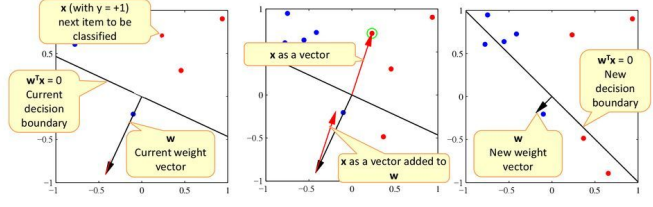
\includegraphics[width=0.75\textwidth]{032}
    \label{fig:032}
\end{center}

The perceptron algorithm guarantees that finds \textbf{some} line that separates the data, but we have no guarantees that the perceptron have found a special line. This will be especially important when we will discuss the difference between the perceptron and the Support Vector Machine.